\documentclass[11pt]{exam}
\usepackage[margin=1in]{geometry}
\pagestyle{plain}
\usepackage{amsmath,amsfonts,amssymb,amsthm,enumerate}
\usepackage{multicol}
\usepackage[]{graphicx}
\usepackage{hyperref}
\usepackage{tikz}
\usepackage{pgfplots}
\usepackage{subfigure}
\usepackage[final]{pdfpages}
\usetikzlibrary{angles,quotes}

\addtolength{\footskip}{2\baselineskip} % to lower the page numbers
\title{\vspace{-0.5in} Math 115 \\ Worksheet Section 4.6 (continued)}
\date{}


% \theoremstyle{definition}
% \newtheorem{problem}{Problem}
\renewcommand{\questionlabel}{\textbf{Problem~\thequestion.}}
% \printanswers

\begin{document}
\maketitle
\vspace{-0.75in}
\begin{questions}
  \question A rectangle has one side of length \(8\)cm. How fast is
    the diagonal changing at the instant when the other side is
    \(6\)cm and increasing at \(3\)cm per minute?
    \begin{solution}
      Let us say \(D\) is the length of the diagonal and \(w\) is then
      length of the changing side. Then, \[
        D^2 = w^2+8^2
      \]
      Taking derivatives, we get \[
       2D \frac{dD}{dt}  = 2w \frac{dw}{dt} \implies \frac{dD}{dt} =
       \frac{w}{D} \cdot \frac{dw}{dt}
      \]
      Then, at the moment \(w = 6\), we have \(D = \sqrt{6^2+8^2} =
      10\) and \(\frac{dw}{dt} = 3\) from the statement of the
      problem. Thus, \[
        \frac{dD}{dt} = \frac{6}{10} \cdot 3 = \frac{9}{10} \text{ cm/min}
      \]
    \end{solution}
    \vspace{0.25in}
  \question Grit, which is spread on roads in winter, is stored in mounds which are in the shape of a cone.  As grit is added to the top of the mound at 2 cubic meters per minute, the angle between the slant side of the cone and the vertical remains $45^\circ$.  How fast is the height of the mound increasing when it is half a meter high?
    \begin{solution}
      Let \(r\) be the radius of the base of the cone, \(h\) be its
      height, and \(V\) be its volume. The statement that the angle of
      the slant side of the cone and 
      the vertical remains \(45^\circ\) tells us that \(\frac{r}{h} =
      \tan(45^\circ) = 1 \implies r = h\). Thus, \[
        V = \frac{1}{3} \pi r^2 h \implies V = \frac{1}{3} \pi h^3
      \]
      Taking derivatives of both sides, we get \[
        \frac{dV}{dt} = \pi h^2 \frac{dh}{dt} \implies \frac{dh}{dt} =
        \frac{dV}{dt} \frac{1}{\pi h^2}
      \]
      Now, from the problem, we know \(\frac{dV}{dt} = 2\) and so,
      when \(h = \frac{1}{2}\), we get \[
        \frac{dh}{dt} = \frac{2}{\pi (1/4)} = \frac{8}{\pi} \text{
          meters per minute}
      \]
    \end{solution}
    \vspace{0.25in}
  \question The London Eye is a large Ferris wheel that has diameter
    \(135\) meters and revolves continuously. Passengers enter the
    cabins at the bottom of the wheel and complete one revolution in
    about 27 minutes. One minute into the ride, a passenger is rising
    at \(0.06\) meters per second. How fast is the horizontal motion
    of the passenger at that moment?
    \begin{solution}
      If the Ferris wheel completes one revolution in 27 minutes, then
      one minute into the ride, a passenger has completed
      \(\frac{1}{27}\)-th of the ride, so they have rotated
      \(\frac{2\pi}{27}\) radians. Let \(x\) be the horizontal
      distance the passenger has traveled and let \(y\) be the
      vertical distance from the center of the Ferris wheel.\\
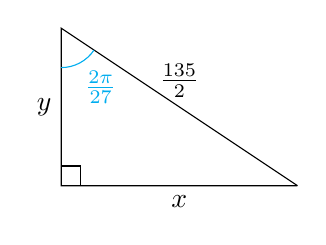
\begin{tikzpicture}[
  my angle/.style={
    every pic quotes/.append style={text=cyan},
    draw=cyan,
    angle radius=0.5cm,
  }]
  \coordinate (C) at (1.5,-1);
  \coordinate (A) at (-1.5,-1);
  \coordinate (B) at (-1.5,1);
  \draw (C) -- node[above] {$\frac{135}{2}$} (B) -- node[left] {$y$} (A) -- node[below] {\(x\)} (C);
  \draw (A) +(.25,0) |- +(0,.25);
  \pic [my angle, ] {angle=A--B--C};
  \node at (-1,0.25) {\textcolor{cyan}{$\frac{2\pi}{27}$}};
\end{tikzpicture}
Now, we know \[
  x^2+y^2 =\left( \frac{135}{2} \right)^2
\]
So, taking derivatives of both sides, we get \[
  2x \frac{dx}{dt} + 2y\frac{dy}{dt} = 0 \implies \frac{dx}{dt} =
  -\frac{y}{x}\cdot \frac{dy}{dt}
\]
Now, one minute into the ride, we know \(\frac{dy}{dt} = -0.06\)
(since our setup has \(y\) decreasing as the passenger moves up this
early in the ride). We also know that \(x = \frac{135}{2} \sin\left(
  \frac{2\pi}{27} \right)\) and \(y = \frac{135}{2} \cos\left(
  \frac{2\pi}{27} \right)\). Plugging this all in, we get \[
  \frac{dx}{dt} = - \frac{\cos\left( \frac{2\pi}{27}
    \right)}{\sin\left( \frac{2\pi}{27} \right)} \cdot (-0.06) =
  0.2532 \text{ meters per second}
\]
    \end{solution}
    \vspace{0.25in}
  \question (Fall 2016 Final Exam) % problem 2
Uri is filling a cone with molten aluminum. The cone is upside-down, so the base is at the top of the cone and the vertex at the bottom, as shown in the diagram. The base is a circular disk with radius 7 cm and the height of the cone is 12 cm.
Recall that the volume of a cone is $\frac{1}{3}A h$, where $A$ is the area of the base and $h$ is the height of the cone (i.e., the vertical distance from the vertex to the base). (Note that the diagram may not be to scale.)
\begin{center}
  \includegraphics[scale=0.4]{aluminium.png}
\end{center}
\begin{enumerate}[(a)]
\item Write a formula in terms of $h$ for the volume $V$ of molten aluminum, in cm$^3$, in the cone if the molten aluminum in the cone reaches a height of $h$ cm.
\item The height of molten aluminum is rising at 3 cm/sec at the moment when the molten aluminum in the cone has reached a height of 11 cm. What is the rate, in cm$^3$/sec, at which Uri is pouring molten aluminum into the cone at that moment?
\item The height of molten aluminum is rising at 3 cm/sec at the moment when the molten aluminum in the cone has reached a height of 11 cm. What is the rate, in cm$^2$/sec, at which the area of the top surface of the molten aluminum is increasing at that moment?
\end{enumerate}
\begin{solution}
  See \href{https://dhsp.math.lsa.umich.edu/exams/115exam3/f16/s2.pdf}{https://dhsp.math.lsa.umich.edu/exams/115exam3/f16/s2.pdf}
\end{solution}
\pagebreak
\question (Winter 2015 Final Exam) % problem 4
Having taken care of Sebastian and sent Erin into the hands of the Illumisqati, King Roderick is pleased that his plan is proceeding well. Our wicked villain decides to relax with a handmade chocolate before he heads to his farmhouse. The process of making the chocolate involves pouring molten chocolate into a mould. The mould is a cone with height 60 mm and base radius 20 mm. Roderick places the mould on the ground and begins pouring the chocolate through the apex of the cone.
\vspace{-1em}
\begin{center}
  \includegraphics[scale=0.4]{chocolate}
\end{center}
\vspace{-1em}
\begin{enumerate}[(a)]
\item Let $g$ be the depth of the chocolate, in mm, as shown in the diagram above. What is the value of g when Roderick has poured a total of 20,000 mm$^3$ of chocolate into the mould? Show your work carefully, and make sure your answer is accurate to at least two decimal places.
\item How fast is the depth of the chocolate in the mould ($g$ in the diagram above) changing when Roderick has already poured 20,000 mm3 of chocolate into the mould if he is pouring at a rate of 5,000 mm$^3$ per second at this time? Show your work carefully and make sure your answer is accurate to at least two decimal places. Be sure to include units.
\end{enumerate}
\begin{solution}
  See \href{https://dhsp.math.lsa.umich.edu/exams/115exam3/w15/s4.pdf}{https://dhsp.math.lsa.umich.edu/exams/115exam3/w15/s4.pdf}
\end{solution}
\question (Winter 2018 Final Exam) % problem 7
A group of meteorologists observe that the sea level is rising by observing a piece of a rock in the sea. Only the tip of the rock is visible, and as the sea water rises, less and less of the rock is above water. Let $h$ and $r$ be the height and radius (in inches), respectively, of the part of the rock that is above the sea. The volume of the rock (in cubic inches) is then given by the formula $V = \frac{\pi}{2} (1+r^2)h$.
\vspace{-1em}
\begin{center}
  \includegraphics[scale=0.4]{rock.png}
\end{center}
\vspace{-0.7em}
The meteorologists notice that, as the level of the sea is rising, the radius and volume of the rock are changing. A year after they started taking the measurements, the radius and height of the rock are 5 and 46 inches, respectively. They notice that at that time, the radius is decreasing at a rate of 0.05 inches per year, which makes the volume change at a rate of 80 cubic inches per year. At what rate is the height of the rock changing at that time? Be sure to include units. Is the height of the part of the rock that is above the sea increasing or decreasing?
\begin{solution}
  See \href{https://dhsp.math.lsa.umich.edu/exams/115exam3/w18/s7.pdf}{https://dhsp.math.lsa.umich.edu/exams/115exam3/w18/s7.pdf}
\end{solution}
\question A 15-ft ladder leaning against a wall begins to slide. How fast is the top of the ladder sliding down the wall at the instant of time when the bottom of the ladder is 9 ft from the wall and sliding away from the wall at the rate of 6 ft/sec?
\\
\begin{center}
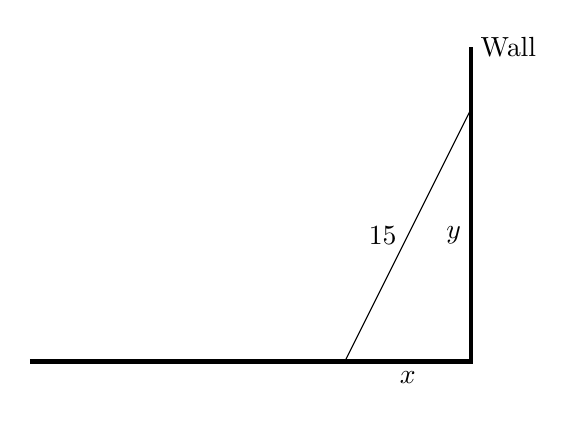
\begin{tikzpicture}[scale =.8]
\draw[ultra thick] (-7, 0)--(0,0)--(0, 5);
\draw (-2,0)--(0,4);
\node[right] at (0, 5) {Wall};
\node[left] at (0, 2) {$y$};
\node [below] at (-1,0) {$x$};
\node at (-1.4, 2) {$15$};
\end{tikzpicture}
\end{center}
\begin{solution}
  \underline{Step 1:} 
Let $x$ be the distance from the bottom of the ladder to the wall and let $y$ be the distance from the floor to the top of the ladder. It is important to recognize that $x$ and $y$ are both functions of time $t$. In other words, as time changes the ladder is slipping, so $x$ and $y$ both change. 
  \\
\underline{Step 2:} From the problem, we see that we are trying to find $\dfrac{dy}{dt}$ when $\dfrac{dx}{dt}=6$ and $x=9$. 
\\
\\\underline{Step 3:} By the Pythagorean theorem, we see that $15^2=x^2+y^2$. 
\\
\\\underline{Step 4:}
\begin{align*}
\frac{d}{dt}(15^2)&=\frac{d}{dt}(x^2+y^2)\\
\implies 0&= 2x\frac{dx}{dt}+2y\frac{dy}{dt}
\end{align*}
\underline{Step 5:} From the original Pythagorean theorem equation, we know when $x =9$ that $15^2 =9^2+y^2$. Therefore, when $x=9$, $y=\pm12$. But for this problem it only makes sense for $y=12$. Now we simply plug in $x=9$, $y=12$, and $\dfrac{dx}{dt}=6$ into the equation in step 4. 
\begin{align*}
0&=2(9)(6)+2(12)\frac{dy}{dt}\\
\implies \frac{dy}{dt}&=-\frac{9}{2}
\end{align*}
So the final answer is that the ladder is sliding down the wall at a rate of $\frac{9}{2}$ ft/sec when $x=9$ and $\frac{dx}{dt}=6$. 
\end{solution}
\question A coffee pot in the form of a circular cylinder of radius 5 in. is being filled with water flowing at a constant rate. If the water level is rising at the rate of 0.7 in./sec, what is the rate at which water is flowing into the coffee pot?
\begin{center}
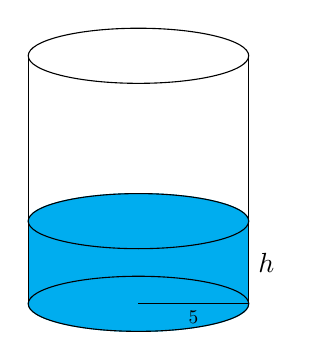
\begin{tikzpicture}[scale =.7]
\filldraw[cyan] (5,.5) ellipse [x radius =2, y radius = .5];
\filldraw[cyan] (5,2) ellipse [x radius =2, y radius = .5];
\filldraw[cyan] (3,.5) rectangle (7,2);
\draw (5,2) ellipse [x radius =2, y radius = .5];
\draw(5,.5) ellipse [x radius =2, y radius = .5];
\draw (5,5) ellipse [x radius =2, y radius = .5];
\draw (3,5)--(3,.5);
\draw (7,5)--(7,.5);
\draw (7,.5)--(5,.5);
\node[below, scale =.7] at (6,.5) {$5$};
\node[right] at (7,1.25) {$h$};
\end{tikzpicture}
\end{center}
\begin{solution}
\underline{Step 1:}
Let $h$ be the height of the water in the coffee pot. Let $V$ be the volume of water in the pot. It is important to recognize that $V$ is a function of $h$ and $h$ is a function of time $t$. In other words, as time changes the height of the water changes and as the height of the water changes the volume of the water changes. 

\underline{Step 2:}  From the problem, we see that $\dfrac{dh}{dt}=.7$ and we are trying to find $\dfrac{dV}{dt}$. 
\\
\\
\underline{Step 3:} $V=(5^2)\pi h\implies V=25\pi h$
\\
\\
\underline{Step 4:} $\frac{dV}{dt}=25\pi \frac{dh}{dt}$
\\
\\
\underline{Step 5:} Trying to find $\dfrac{dV}{dt}$ and we know $\dfrac{dh}{dt}=.7$. So plugging into the equation from step 4 we get:
\begin{align*}
\frac{dV}{dt}=25\pi (.7)\approx 54.98
\end{align*}
The final answer is $54.98$ in.$^3$/sec
\end{solution}
\question Suppose we have a constantly changing rectangular box with fixed volume of $100\text{ in}^3$ and a square base where the sides of the base are increasing by $5$ inches every second. If this necessarily flexible material costs $\$10, \$20,$ and $\$30$ per square inch, for the top, bottom, and sides, respectively, then find the rate of change of the cost when the sides of the base are $10$ inches.
\begin{center}
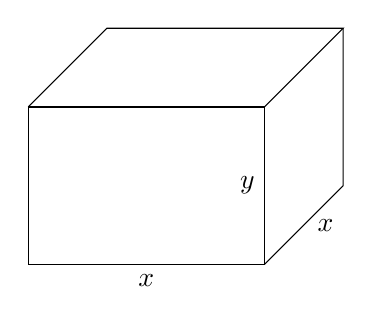
\begin{tikzpicture}
\draw (-4,0)--(-1,0)--(-1,2)--(-4,2)--(-4,0);
\draw (-4,2)--(-3,3)--(0,3)--(-1,2);
\draw (0,3)--(0,1)--(-1,0);
\node[below] at (-2.5,0) {$x$};
\node[left] at (-1,1) {$y$};
\node[right] at (-.45, .5) {$x$};
\end{tikzpicture}
\end{center}
\begin{solution}
 \underline{Step 1:} Let $x$ be the length of a side of the base of the box, $y$ be the height of the box, $V$ be the volume of the box and $C$ be the total material cost of the box. It is important to recognize that $V$ and $C$ are both functions of $x$ and $y$, and $x$ and $y$ are both functions of time $t$. 

\underline{Step 2:} We are trying to find $\dfrac{dC}{dt}$ when $x=10$ given that the material costs $\$10, \$20,$ and $\$30$ per square inch, for the top, bottom, and sides, respectively and that $\dfrac{dx}{dt}=5$ and $V=100$ is fixed. 
\\
\\\underline{Step 3:} \begin{align*}
100&=V=x^2y\\
C&=10x^2 +20x^2 +30(4)xy=30x^2+120xy
\end{align*}
\underline{Step 4:}
\begin{align*}
0&=2x\frac{dx}{dt}y+x^2\frac{dy}{dt}\\
\frac{dC}{dt}&=60x\frac{dx}{dt}+120\frac{dx}{dt}y+120x\frac{dy}{dt}
\end{align*}
\underline{Step 5:} From the volume equation, when $x=10$ we have that $100=10^2y$, thus $y=1$. So now we plug in $x=10$, $y=1$, and $\dfrac{dx}{dt}=5$ into the equations in step 4 and solve for $\dfrac{dC}{dt}$. 
\begin{align*}
0&=2(10)(5)(1)+(10)^2\frac{dy}{dt}\implies \frac{dy}{dt} = -1\\
\frac{dC}{dt}&=60(10)(5)+120(5)(1)+120(10))(-1)=2400
\end{align*}
Therefore, the final answer is that the rate of change of the cost when the sides of the base are 10 inches is equal to $2400$ dollars/sec. 
\end{solution}
\pagebreak
\question \textbf{Challenge:} Suppose that water is flowing out of a hole at the bottom of a cone into a cylinder located below the bottom of the cone. Suppose that the height of the water in the cone is decreasing at a constant rate of $2\ cm/sec$. The cone has radius $10\ cm$ and height $20\ cm$. The cylinder has radius $30\ cm$ and height $70\ cm$. For simplicity, assume that as soon as water leaves the hole of the cone it instantaneously goes into the cylinder. In other words, it takes 0 time for the water to fall from the hole into the cylinder. What is the rate of change of the height of the water in the cylinder when the height of the water in the cone is $4\ cm$? \textbf{(Hint: Use Similar Triangles)}
\\
% \\\textbf{Solution:}
% \\
% \\\underline{Step 1:} Let $h_{1}$ be the height of the water in the cone and let $h_{2}$ be the height of the water in the cylinder. Let $r$ be the radius of the cone of water contained in the cone. In the figure below, $r$ is in green. Let $V_{1}$ be the volume of the water in the cone. Let $V_{2}$ be the volume of water in the cylinder. Notice $h_{1}$, $h_{2}$ and $r$ are functions of time. $V_{1}$ is a function of $h_{1}$ and $r$. $V_{2}$ is a function $h_{2}$. 
\begin{center}
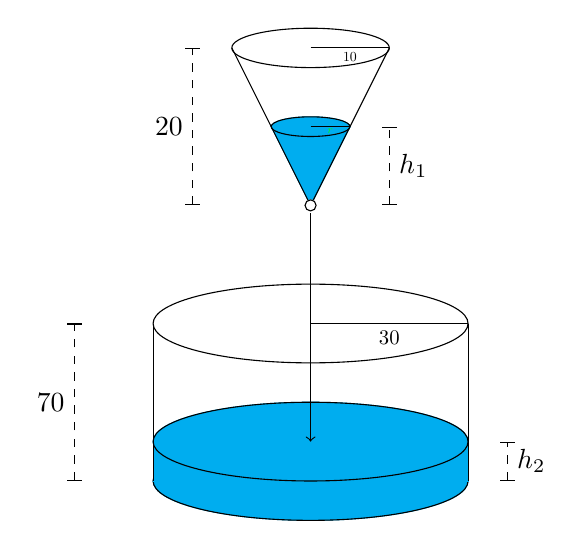
\begin{tikzpicture}
\filldraw[cyan] (5,.5) ellipse [x radius =2, y radius = .5];
\draw (5,.5) ellipse [x radius =2, y radius = .5];
\filldraw[cyan](3,.5)  rectangle (7,1);
\filldraw[cyan] (5,1) ellipse [x radius =2, y radius = .5];
\draw (5,1) ellipse [x radius =2, y radius = .5];
\filldraw[cyan] (5,4)--(4.5,5)--(5.5,5)--(5,4);
\filldraw[cyan] (5,5) ellipse [x radius =.5, y radius = .125];
\draw (5,5) ellipse [x radius =.5, y radius = .125];
\draw (5,6) ellipse [x radius =1, y radius = .25];
\draw (4,6)--(5,4)--(6,6);
\draw (5,2.5) ellipse [x radius =2, y radius = .5];
\filldraw[white] (5,4) circle(2pt);
\draw (5,4) circle(2pt);
\draw[->] (5,3.9)--(5,1);
\draw[dashed,|-|] (3.5,4)--(3.5,6);
\node[left] at (3.5,5) {$20$};
\draw[dashed,|-|] (6,4)--(6,5);
\node[right] at (6,4.5) {$h_{1}$};
\draw (5,6)--(6,6);
\node[below, scale = .5] at (5.5, 6) {$10$};
\draw (5, 5)--(5.5,5);
\node[green, scale = .4] at (5.25, 4.94) {$r$};
\draw[dashed,|-|] (2,.5)--(2,2.5);
\node[left] at (2,1.5) {$70$};
\draw[dashed,|-|] (7.5,.5)--(7.5,1);
\node[right] at (7.5,.75) {$h_{2}$};
\draw (5,2.5)--(7,2.5);
\node[below, scale =.75] at (6,2.5) {$30$};

\draw (3,2.5)--(3,.5);
\draw (7,2.5)--(7,.5);
\end{tikzpicture}
\end{center}
\begin{solution}
 \underline{Step 1:} Let $h_{1}$ be the height of the water in the cone and let $h_{2}$ be the height of the water in the cylinder. Let $r$ be the radius of the cone of water contained in the cone. In the figure below, $r$ is in green. Let $V_{1}$ be the volume of the water in the cone. Let $V_{2}$ be the volume of water in the cylinder. Notice $h_{1}$, $h_{2}$ and $r$ are functions of time. $V_{1}$ is a function of $h_{1}$ and $r$. $V_{2}$ is a function $h_{2}$. 

\underline{Step 2:} We are trying to find $\dfrac{dh_{2}}{dt}$ when $h_{1} = 4$ given that $\dfrac{dh_{1}}{dt}=-2$. 
\\
\\
\underline{Step 3:} From the figure we see that $V_{1} = \frac{1}{3}\pi r^2h_{1}$ and $V_{2} = \pi(30)^2h_{2}$. Using similar triangles, we can find the relationship between $r$ and $h_{1}$. 
\\
\begin{center}
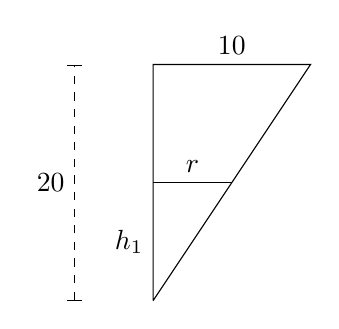
\begin{tikzpicture}
\draw (0,0)--(0,3)--(2,3)--(0,0);
\draw (0,1.5)--(1,1.5);
\draw[dashed, |-|] (-1,0)--(-1,3);
\node[left] at (-1,1.5) {$20$};
\node[above] at (1,3) {$10$};
\node[above] at (.5,1.5) {$r$};
\node[left] at (0, .75) {$h_{1}$};
\end{tikzpicture}
\end{center}
We find that $\frac{h_{1}}{r}=\frac{20}{10}$. Rewriting this we have that $h_{1}=2r$. 
\\
\\
\underline{Step 4:} There are three equations to differentiate with respect to time.
\begin{align*}
\frac{dV_{1}}{dt}&=\frac{d}{dt}\left(\frac{1}{3}\pi r^2h_{1}\right)\\
&=\frac{1}{3}\pi2r\frac{dr}{dt}h_{1}+\frac{1}{3}\pi r^2\frac{dh_{1}}{dt}\\
&=\frac{\pi}{3}\left(2h_{1}r\frac{dr}{dt}+r^2\frac{dh_{1}}{dt}\right)\\
\\
\frac{dV_{2}}{dt}&=900\pi\frac{dh_{2}}{dt}
\\
\\
\frac{dh_{1}}{dt}&=2\frac{dr}{dt}
\end{align*}
\underline{Step 5:} From the set up of the problem, the rate at which the volume of water in the cone is decreasing is equal to the rate at which the volume of the water in the cylinder is increasing. Therefore, $\dfrac{dV_{2}}{dt}=-\dfrac{dV_{1}}{dt}$. We are trying to find $\dfrac{dh_{2}}{dt}$ when $h_{1}= 4$. From step 3, we see that when $h_{1} = 4$, we have $r=2$.  
\\
\\Now we plug in $h_{2} = 4$, $r=2$, and $\dfrac{dh_{1}}{dt}=-2$ into the equations in step 4. 
\begin{align*}
-2=2\frac{dr}{dt}\implies \frac{dr}{dt}=-1
\end{align*}
\begin{align*}
\frac{dV_{1}}{dt}&=\frac{\pi}{3}(2(4)(2)(-1)+(2)^2(-2))=-8\pi\\
\implies 8\pi &= -\frac{dV_{1}}{dt}=\frac{dV_{2}}{dt}=900\pi\frac{dh_{2}}{dt}\\
\implies \frac{dh_{2}}{dt}&=\frac{2}{225}
\end{align*}
\\
Therefore, the rate of change of the height of the water in the cylinder when the height of the water in the cone is $4\ cm$ is equal to $\dfrac{2}{225}$ cm/sec.

\end{solution}
\end{questions}
\end{document}
%%% Local Variables:
%%% mode: latex
%%% TeX-master: t
%%% End:
